\chapter{Multi-version Software Updates}
\label{chap:safe-updates}

% Software updates are an integral part of the software maintenance
% process, with new software versions being released on a continuous
% basis.  Unfortunately, software updates often result in failures,
% which makes many users reluctant to incorporate the latest patches
% made available by developers.  As a result, users rely instead on
% outdated versions, which despite their relative stability, miss recent
% features and bug fixes and may be plagued by security vulnerabilities.

% One of the main reasons for which users hesitate to install updates is
% that a significant number of them result in failures.  It is only too
% easy to find examples of updates that fix a bug or a security
% vulnerability only to introduce another problem in 
% the code. Our goal is to improve the software update
% process in such a way as to encourage users to upgrade to the latest
% software version, without sacrificing the stability of the older
% version.

Multi-version execution can be used to improve the reliability of updated
software by running multiple different versions (revisions) in parallel,
discarding one (or more) versions in case of failure. The potential problem
of such approach is that we might run out of alive versions given multiple
crash bugs located in different parts of the application. We tackle this
problem by combining a multi-version execution with a failure recovery
mechanism which takes an advantage of the similarity between consecutive
software versions.

% We tackle this problem using a simple but effective multi-version
% based approach.  Whenever a new update becomes available, instead of
% upgrading the software to the new version, we run the new version in
% parallel with the old one; by carefully coordinating their executions
% and selecting the behaviour of the more reliable version when they
% diverge, we create a more secure and dependable multi-version
% application.

We implemented this approach in a prototype system called \mx, which
targets crash bugs in Linux applications
%running on multi-core processors.
\mx allows a new and an old version of an application to
run concurrently, without requiring any
modifications to the application itself or the operating system, nor any
input from the user. To achieve this goal, \mx combines static and
dynamic techniques: it uses static analysis at the binary-level to
construct mappings between the old and the new versions, and synchronizes
execution of the two versions at the system call level, using system call
interposition and synchronisation.  When one of the versions crashes, \mx
transparently restarts it via a lightweight checkpointing mechanism and often
allows it to survive the bug by using the code of the other version.

% We evaluate \mx by showing that it can successfully survive crashes in
% several real applications, specifically several \coreutils utilities and
% two popular servers, \lighttpd and \redis.

%Software systems are constantly evolving, with new versions and
%patches being released on a continuous basis.  Unfortunately, software
%updates present a high risk, with many releases introducing new bugs
%and security vulnerabilities.

%% Applicable in a variety of scenarios, example of one such
%% application might be the desktop and office software where users
%% care about reliability more than performance or efficiency.
%% Examples of such scenarios are provided further in this
%% section. Another application might be the software systems where
%% reliability is critically important, such as web servers,
%% databases, \etc

%% We also believe, that the proposed approach might facilitate and
%% improve the \emph{continuous deployment} technique. While this
%% technique has been frequently proposed and advocated in the
%% software engineering community because it encourages
%% experimentation, innovation, and rapid
%% iteration~\cite{johnson2009,harmess2009,linden2009}, its use is
%% still limited since updates may introduce new bugs and security
%% vulnerabilities.  We believe that our approach provides all the
%% benefits of continuous deployment without compromising software
%% reliability.

To motivate our approach, we present a real scenario involving
\lighttpd, which is representative of one type of applications which
could benefit from our approach, namely server applications with
stringent security and availability requirements.


%% that achieves high-scalability, without sacrificing
%% standards-compliance and security having a small-memory footprint
%% and a small CPU load.  As a result, \lighttpd is
\lighttpd\footnote{\url{http://www.lighttpd.net/}} is a popular open-source 
web-server used 
%(either alone or in conjunction with other web-servers)
by several high-traffic websites such as Wikipedia and Xkcd.
Despite its popularity, crash bugs are still a common
occurrence in \lighttpd, as evident from its bug tracking
database.\footnote{\url{http://redmine.lighttpd.net/issues/}}  Below
we discuss one such bug, which our approach could successfully
eliminate.

%% In October 2008, a bug was reported in \lighttpd affecting the HTTP
%% ETag
%% functionality\footnote{\url{http://redmine.lighttpd.net/issues/1800}}.
%% An ETag a fingerprint assigned by a web server to a specific version
%% of a web resource, which can be used to quickly determine if the
%% resource has changed.  The bug in \lighttpd was that invalid ETags
%% were generated when compression was used.  The bug was fixed in
%% revision
%% 2386\footnote{\url{http://redmine.lighttpd.net/projects/lighttpd/repository/revisions/2386}},

% April 9th 2009
In April 2009, a patch was
applied\footnote{\url{http://redmine.lighttpd.net/projects/lighttpd/repository/revisions/2438}}
to \lighttpd's code related to the HTTP ETag functionality.  An ETag
is a unique string assigned by a web server to a specific version of a
web resource, which can be used to quickly determine if the resource
has changed.  The patch was a one-line change, which discarded the
terminating zero when computing a hash representing the ETag.  More
exactly, line 47 in \textstt{etag.c}:

\begin{lstlisting}[numbers=none,breaklines=true,xleftmargin=0pt]
for (h=0, i=0; i < etag->used; ++i) h = (h<<5)^(h>>27)^(etag->ptr[i]);
\end{lstlisting}
\noindent was changed to:
\begin{lstlisting}[numbers=none,breaklines=true,xleftmargin=0pt]
for (h=0, i=0; i < etag->used@-1@; ++i) h = (h<<5)^(h>>27)^(etag->ptr[i]);
\end{lstlisting}

This correctly changed the way ETags are computed, but unfortunately,
it broke the support for compression, whose implementation depended on
the previous computation.  More precisely, \lighttpd's support for HTTP
compression uses caching to avoid re-compressing files which have not
changed since the last access.  To determine whether the cached
file is still valid, \lighttpd internally uses ETags.  Unfortunately,
the code implementing HTTP compression did not consider the case when
ETags are disabled.  In this case, \textstt{etags->used}
is \textstt{0}, and when the line above is
executed, \textstt{etag->used-1} underflows to a very large value, and
the code crashes while accessing \textstt{etag->ptr[i]}.
Interestingly enough, the original code was still buggy (it always
returns zero as the hash value, and thus it would never re-compress
the files), but it was not vulnerable to a crash. %denial of service
                                                  %attack.

%% \begin{figure}
%% \centering
%% \includegraphics[width=0.9\columnwidth]{safe-updates/figures/lighttpd-scenario}
%% \caption{Crash bug \#2169 from {\footnotesize \texttt{lighttpd}}.}
%% \label{fig:lighttpd-history}
%% \end{figure}

% 8 March
The segfault was diagnosed and reported in March
2010\footnote{\url{http://redmine.lighttpd.net/issues/2169}} and fixed
at the end of April
2010,\footnote{\url{http://redmine.lighttpd.net/projects/lighttpd/repository/revisions/2723}}
more than one year after it was introduced.  
%The history is depicted graphically in Figure~\ref{fig:lighttpd-history}.  
The bottom line is
that for about one year, users affected by this buggy patch
essentially had to decide between%
\begin{inparaenum}[(1)]
\item incorporating the new features
and bug fixes added to the code, but being vulnerable to this crash
bug, and
\item giving up on these new features and bug fixes and using
an old version of \lighttpd, which is not vulnerable to this bug.
\end{inparaenum}
Note that this is particularly true for the eleven-month period
between the time when the bug was introduced and the time it was
diagnosed, since during this period most users would not know how to
change the server's configuration to avoid the crash.

%% The original code, which can be seen in Listing~\ref{lst:2437}, makes the
%% \texttt{i < etag->used} comparison (line 4). Because both \texttt{i} and
%% \texttt{etag->used} are $0$, the condition \texttt{0 < 0} does not hold and
%% the loop body will never be executed.

%% The affected code can be seen in Listing~\ref{lst:2438}. Here, the condition
%% has been changed and comparison has now the form \texttt{i < etag->used-1}.
%% When executing, the \texttt{etag->used} variable will underflow and condition
%% \texttt{0 < 4294967295} will be true. Therefore, the loop body will be
%% executed and access to \texttt{etag->ptr[0]} will result in segmentation
%% fault.

Our approach provides users with a third choice; when a new version
arrives, instead of replacing the old version, we run both versions in
parallel. In our example, consider that we are using \mx to run a
version of \lighttpd from March 2009.  When the buggy April 2010 version
is released, \mx runs it in parallel with the old one.  As the two
versions execute:

\begin{itemize}
\item As long as the two versions have the same external behaviour (\eg they 
write the same values into the same files, or send the same data over
the network), they are run side-by-side and \mx ensures that they act
as one to the outside world (see \S\ref{sec:mxm});

\item{When one of the versions crashes (\eg the new version executes 
the buggy patch), \mx will patch the crashing version at runtime using
the behaviour of the non-crashing version 
(see \S\ref{sec:rem})}.  In this way, \mx can successfully survive
crash bugs in both the old and the new version, increasing the
reliability and availability of the overall application;\looseness=-1

\item When a non-crashing divergence is detected, \mx will discard one of
the versions (by default the old one, but other heuristics can be
used).  The other version can be later restarted at a convenient
synchronisation point (\eg at the beginning of the dispatch loop of
a network server).

\end{itemize}

%% When the two versions diverge because of the newly introduced bug
%% and the April 2010 version crashes, \mx will patch the crashing
%% version at runtime using the behaviour of the non-crashing
%% version. While the recovered version continues to execute, \mx uses
%% the correctly executing March 2009 version as an oracle to ensure
%% that its behaviour is correct. When any divergence is detected, \mx
%% will discard the recovered version and continue using only the old
%% version to ensure correctness. If the divergence is detected
%% during the normal execution, \mx will by default prefer the
%% behaviour of the newer version, but other heuristics can be used as
%% well.

From the user's point of view, this process is completely transparent
and does not cause any interruption in service. In our example, this
effectively eliminates the bug in \lighttpd, while still allowing
users to use the latest features and bug fixes of the recent versions.

%In our proposed approach, when a new version arrives, instead of
%replacing the old version, we run both versions in parallel.  As more
%versions arrive, we execute them in parallel with the existing ones,
%until all available resources have been exhausted, at which point we
%discard some of the versions according to some strategy.

%In our example, consider a system that is running a version
%of \lighttpd from March 2009.  When the buggy April 2010 version is
%released, our system runs it in parallel with the old one.  As the two
%versions execute, the system checks that their external behaviour is
%identical (\eg they write the same values into the same files, or send
%the same data over the network).  When the two versions diverge, the
%divergence is resolved in the favour of the more reliable version.  In
%particular, if one of the two versions crashes, the behaviour of the
%non-crashing version is used, and the other version is transparently
%modified to survive the crash. (Note that the last point is of key
%importance, as the success of our technique depends on having all
%versions running at all times.)  If the system cannot determine which
%behaviour is correct, a simple heuristic can be used, such as always
%preferring the behaviour of the newer version.  In our example, this
%effectively eliminates the bug in \lighttpd, while still allowing
%users to use the latest features and bug fixes of the recent versions.

%Figure~\ref{fig:lighttpd-history}, 


%% Bug 1800: not really using it
%%
%% The bug \#1800 was also related to the HTTP compression and ETag functionality; in
%% particular, invalid ETags were generated for compressed variants of the same
%% resource. The solution for this bug did not consider the situation when
%% ETag support is completely disabled. However, due to an incorrect implementation
%% of ETag hash function, this bug remain undetected until the revision
%% \texttt{2438} when ETag hash function has been fixed.

%% The \texttt{mod\_compress} module implementing the HTTP compression support
%% uses caching to avoid re-compression of files which has been already
%% compressed in the past. To determine whether the cached file is still valid,
%% \texttt{mod\_compress} internally uses ETag stored along with the file.

%% Then, when request for a file is made, \texttt{mod\_compress} module
%% implementation shown in Listing~\ref{lst:2386} first reads the physical file
%% along with its ETag (line 4) and tries to match this ETag with the original
%% one (line 9). However, if ETag support has been disabled, the ETag of the
%% physical file would be empty.

%% \begin{lstlisting}[label=lst:2386,caption={Refactored failing version of the function}]
%% PHYSICALPATH_FUNC(mod_compress_physical) {
%%   stat_cache_entry *sce = NULL;
%%   ...
%%   if (HANDLER_ERROR == stat_cache_get_entry(srv, con, con->physical.path, &sce)) {
%%     ...
%%   }
%%   ...
%%   /* try matching original etag of uncompressed version */
%%   etag_mutate(con->physical.etag, sce->etag);
%%   ...
%% }
%% \end{lstlisting}

%% The original code, which can be seen in Listing~\ref{lst:2437}, makes the
%% \texttt{i < etag->used} comparison (line 4). Because both \texttt{i} and
%% \texttt{etag->used} are $0$, the condition \texttt{0 < 0} does not hold and
%% the loop body will never be executed.

%% The affected code can be seen in Listing~\ref{lst:2438}. Here, the condition
%% has been changed and comparison has now the form \texttt{i < etag->used-1}.
%% When executing, the \texttt{etag->used} variable will underflow and condition
%% \texttt{0 < 4294967295} will be true. Therefore, the loop body will be
%% executed and access to \texttt{etag->ptr[0]} will result in segmentation
%% fault.

%% \begin{lstlisting}[label=lst:2437,caption={Original version of \texttt{etag\_mutate} function}]
%% int etag_mutate(buffer *mut, buffer *etag) {
%%   size_t i;
%%   uint32_t h;
%%   for (h=0, i=0; i < etag->used; ++i) h = (h<<5)^(h>>27)^(etag->ptr[i]);
%%   buffer_reset(mut);
%%   buffer_copy_string_len(mut, CONST_STR_LEN("\""));
%%   buffer_append_long(mut, h);
%%   buffer_append_string_len(mut, CONST_STR_LEN("\""));
%%   return 0;
%% }
%% \end{lstlisting}

%% \begin{lstlisting}[label=lst:2438,caption={Modified version of \texttt{etag\_mutate} function}]
%% int etag_mutate(buffer *mut, buffer *etag) {
%%   size_t i;
%%   uint32_t h;
%%   for (h=0, i=0; i < etag->used-1; ++i) h = (h<<5)^(h>>27)^(etag->ptr[i]);
%%   buffer_reset(mut);
%%   buffer_copy_string_len(mut, CONST_STR_LEN("\""));
%%   buffer_append_long(mut, h);
%%   buffer_append_string_len(mut, CONST_STR_LEN("\""));
%%   return 0;
%% }
%% \end{lstlisting}

\section{Prototype}
\label{sec:mx}

%% \begin{figure}[t!]
%% \centering
%% \includegraphics[width=\columnwidth]{safe-updates/figures/overview}
%% \caption{A platform running both conventional and multi-version
%%   applications.}
%% \label{fig:mx-platform}
%% \end{figure}

We have implemented our approach in a prototype system called \mx,
targeted at multi-core processors running Linux.  Currently, \mx
supports two versions run in parallel. The system works directly on
application binaries, making it easy to deploy it and possibly integrate
it with existing software package managers such as \texttt{apt} or
\texttt{yum}.

%Figure~\ref{fig:mx-platform} shows a platform running \mx, on which
On a platform using \mx, conventional (\ie unmodified) applications
and multi-version (\mv) applications run side by side.  The key
property that must hold on such a platform is that without purposely
trying to do so, applications should not be able to distinguish
between conventional and \mv applications running on the platform. In
particular, the multiple versions of an \mv application should appear
as one to any other entity interacting with them (\eg user, operating
system, other machines).  Furthermore, \mv applications should be more
reliable and secure than their component versions, and their
performance should not be significantly degraded.

To achieve these goals, our prototype \mx employs several different
components, as shown in the architectural overview of
Figure~\ref{fig:design}.  The input to \mx consists of the binaries of
two versions of an application, which we will refer to as 
\textit{the old version}---the one already running on the system, and 
\textit{the new version}---the one newly released.


These two binaries are first statically analysed by the \sea (Static
Executable Analyser) component, which constructs a mapping from the
control flow graph (CFG) of the old version to the CFG of the new
version (\S\ref{sec:sea}).  The two versions are then passed to \mxm
(Multi-eXecution Monitor), whose job is to run the two versions in
parallel, synchronise their execution, virtualise their interaction
with the outside environment, and detect any divergences in their
external behaviour (\S\ref{sec:mxm}).  Once a divergence is detected,
it is resolved by \rem (Runtime Execution Manipulator), which selects
between the available behaviours, and resynchronises the two versions
after the divergence (\S\ref{sec:rem}).

The system prototype has been implemented in C with a small amount of
assembly, and the current version has approximately \mxSLOC source
lines of code. The implementation currently supports Linux kernels
3.2.0 and above, running x86 and x86-64 architectures.

The rest of this section describes the main \mx system components and
their implementation in more detail, and discusses how they work
together to support safe software updates.

\begin{figure}[t!]
\begin{center}
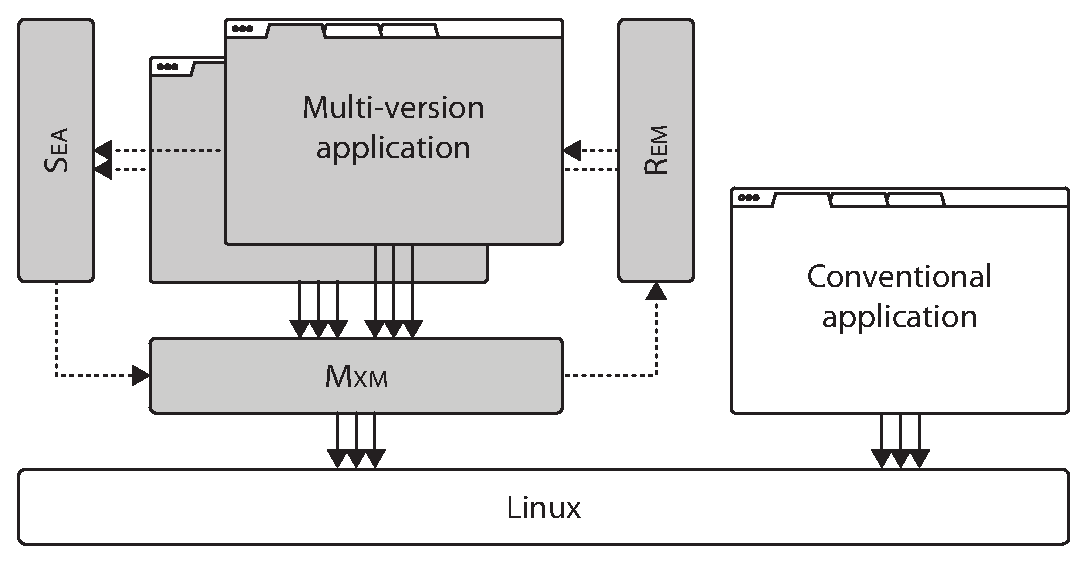
\includegraphics[width=0.6\columnwidth]{safe-updates/figures/architecture}
\caption{\mx system architecture.  
%% The main components of \mx
%%   are \sea (Static Executable Analyser), \mxm (Multi-eXecution
%%   Monitor), and \rem (Runtime Execution Manipulator).
}
\label{fig:design}
\end{center}
\end{figure}


\subsection{System call interposition}
\label{sec:mxm}

One of the main components of our multi-version execution environment
is the \mxm monitor.  \mxm's main jobs are to run the two versions
concurrently, mediate their interaction with the outside world,
synchronise their executions, and detect any divergences in their
external behaviour. \mxm works by intercepting all system calls issued
by each application version, and manipulating them to ensure that the
two versions are executed in a synchronised fashion and act as one to
the outside world.

\mxm provides functionality similar to conventional virtual machine monitors.
Whenever the MV application is executed, the \mxm connects to the two
application versions running in parallel, intercepting their kernel system
calls.  \mxm ensures that the two versions act as one to the outside world by
mediating access to the underlying operating system to achieve complete
isolation of the running application from other application instances as well
as from the external environment, making sure the combined application versions
act as one to the outside world.  The environment controlled by the monitor
consists mainly of a restricted file system access, socket interceptors and
signal handlers.

\subsubsection{System call interception}

\mxm is implemented using the  \ptrace interface provided by the Linux
kernel.  This interface, often used for application debugging, allows
simple deployment (without any need for compile-time instrumentation)
and makes the monitor itself lightweight since it is running as a
regular unprivileged process.  \mxm is similar in operation to previous
monitors whose goal is to synchronise applications at the level of system
calls such as \orchestra~\cite{orchestra09}, PLR~\cite{shye2009} or
\tachyon~\cite{tachyon12}.

\mxm runs each version in a separate child process, intercepting all
their system calls.  When a system call is intercepted in one version,
\mxm waits until the other version also performs a system call.  With
a pair of system calls in hand (one executed by the old version, and
one by the new version), \mxm compares their types and arguments.  If
they differ, \mxm has detected a divergence and invokes the \rem
component to resolve it (\S\ref{sec:rem}).

Otherwise, if the two versions perform the same system call with the
same arguments, \mxm virtualises their interaction with the
environment.  If the operation performed by the system call has no
side effects and does not involve virtualised state (\eg
\lstinline`sysinfo`), \mxm allows both processes to execute it
independently.  Otherwise, it executes the system call on their
behalf and copies its results into the address spaces of both
versions.

\mxm must also enforce deterministic execution across versions. This
consists mainly of intercepting instructions that may produce
non-deterministic results, and returning the same result in both
versions.  Examples of such non-deterministic operations include
random number generators (\eg read calls to \lstinline`/dev/[u]random`),
date and time (\eg read calls to \lstinline`/etc/localtime`), and access
to files and network (\eg file descriptor consistency).  Note that
non-deterministic effects resulting from allocating memory objects at
different addresses in memory or randomly arranging memory areas via
address space layout randomisation (ASLR) do not pose any
problems: \mxm understands the semantics of individual system calls and
rather than directly comparing memory addresses (which might be
different in each executed version), it compares the actual values
stored at those memory locations. \mxm supports both memory buffers (by
comparing the actual buffer content) as well as data structures
referenced by pointers (including nested ones).
 
Since \mxm fully controls executing programs intercepting all their system
calls, it can ensure that both programs have the same view of their
environment. Whenever the monitored process makes a system call, \mxm is
notified twice---first before, then after the call has been executed.  When a
\ptrace event is raised (\eg a new child process has been started), the monitor
is notified as well.  Due to internal limitations of the \ptrace interface,
once the system call has been made, it cannot be skipped, so when \mxm wants to
execute the call on behalf of its child processes, it simply replaces it with a
system call that does not change the system state (\lstinline`getpid` in our
case).

There are several challenges that we encountered while implementing
\mxm.  First, \mxm must partly understand the semantics of 
system calls.  For example, many system call parameters use complex
(often nested) structures with complicated semantics to pass values to
the operating system kernel, as in the case of \lstinline`ioctl` or
\lstinline`futex`.  To be able to compare the parameters of
these system calls and copy back their results, \mxm needs to
understand the semantics of these structures.  However, there are only
a relatively small number of system calls in Linux, and once the support
for handling them is implemented, it can be reused across applications.
\mxm currently implements \syscallsImplemented system calls (out of the
\syscallsTotal provided by Linux x86-64 3.1.9), which was enough to
allow us to run \mx on our benchmarks
(\S\ref{sec:reliability-evaluation}).

Second, the arguments of a system call are often passed through pointers,
which are only valid in the application address space, which is not directly
available to \mxm.  Therefore, \mxm needs to copy the contents pointed to by
these structures to its own address space in order to perform their
comparison.  The \ptrace interface on x86-64 only allows to copy one quadword
per system call, which is very expensive. Previous approaches either used
various ad-hoc optimisations~\cite{orchestra09} such as named pipes or shared
memory with custom shellcode, or a modified kernel~\cite{tachyon12} to
overcome this limitation. Instead, \mxm uses \emph{cross memory attach}, a new
mechanism for fast interprocess communication which has been recently added to
the Linux kernel~\cite{crossmemoryattach}.  This mechanism provides two new
system calls---\lstinline`process_vm_readv` and
\lstinline`process_vm_writev`---which allows the tracer to directly access the
memory space of the tracee using an interface similar to the \lstinline`readv`
and \lstinline`writev` system calls without any additional overhead.

Third, because the structures passed as arguments to system calls often have
variable size, \mxm also needs a fast way to allocate and deallocate memory
for them in order to minimise the overall overhead imposed by our system.  For
this purpose, \mxm uses a region-based memory allocator~\cite{memory-pools},
namely the \textsf{obstack}
library,\footnote{\url{http://www.gnu.org/software/hello/manual/libc/Obstacks.html}}
which is part of the \gnu C Library.  Each monitored process has its own
region, which is used for allocating memory to store the copy of the process'
system call arguments

\subsubsection{Multi-process and multi-threaded applications}

Finally, a particular challenge arises in the context of multi-process and
multi-threaded applications.  Using a single monitor instance to intercept both
versions and their child processes (or threads) would eliminate any advantage
that these applications derive from using concurrency.  Therefore, \mxm uses a
new monitor thread for each set of child processes (or threads) spawned by the
application.  For instance, if the old and new versions each have a parent and
a child process, then \mxm will use two threads: one to monitor the parent
processes, and one to monitor the child processes in each version.

Due to limitations of the \ptrace interface (which was not designed to be used
in a multi-process or multi-threaded environment), handing the control of any
child processes being spawned by the application over to a new monitoring
thread is somewhat complicated.  In \mxm we adopt a solution similar to
Orchestra~\cite{orchestra09}.  When a new child process is spawned, we let the
parent monitoring thread to supervise its execution until the first system
call.  Then, we replace this system call with a \lstinline`pause` system call,
disconnect the parent monitor (which causes a \lstinline`SIGCONT` signal to be
sent to all new child processes), and spawn a new monitoring thread which
immediately reconnects to the new child process, restores its original system
call, and resumes its execution.

\mxm does not enforce deterministic execution across multiple versions of
multi-threaded programs (which may diverge if race conditions can lead
to different external behaviour across executions), although we could
overcome this limitation by adopting \varan's solution
(\S\ref{sec:threading}).

%% \mxm also performs a series of optimisations to decrease performance
%% overhead, such as allowing certain files with read-only permissions
%% to be opened directly by the process. 

\subsubsection{Environment virtualisation}

To improve I/O performance and decrease virtualisation overhead,
processes are allowed to open files with read-only permissions
directly, while files with write permissions are opened by the monitor
itself.  This imposes another problem as file descriptors assigned to
these files are not necessarily the same in each version (\eg due to
scheduling non-determinism). Therefore, \mxm needs to virtualise
these file descriptors.

Whenever the monitored process opens a file with read-only permissions, a
new virtual file descriptor is assigned to this file together with the
mapping to a real file descriptor for each version. This virtual file
descriptor is then sent to each version. When a system call is made
using this virtual file descriptor, \mxm replaces it with the real
file descriptor before executing the system call. The actual file
operation is then executed by the process itself avoiding any memory
copying by \mxm.

A similar approach is also used for virtualisation of process,
group, parent and child identifiers.  Whenever a process tries to obtain
the actual ID, \mxm replaces this with a virtual ID and keeps the
mapping between the real and the virtual ID. When a process invokes a
system call using this ID as an argument (\eg \lstinline`kill`), the
virtual ID is replaced with the actual ID before executing the system
call.

%% \paragraph{Para-virtualisation interface and binary translation.}
%% Furthermore, we plan to combine this API with a binary translation
%% approach~\cite{binary-translation}, that will allow to dynamically
%% replace certain system calls with more efficient \emph{monitor
%% call} instructions.  The binary translation could be also used to
%% dynamically replace code components that have been proved to be
%% safe and do not need to be replicated across multiple versions (\eg
%% using static verification during compilation, using traces of
%% previous execution, using runtime heuristics).


%% \paragraph{Future work}

%% The \texttt{ptrace} interface allows us to easily monitor the program
%% execution without any compile-time instrumentation.  The main downside
%% of this approach is a relatively high overhead.  This is especially
%% true for I/O intensive applications, as they require frequent
%% transfers of large portions of the application memory space to the
%% monitor process. This overhead could be eliminated by directly
%% accessing the process memory space.

%% The existing prototype implementation of \textsc{Mxm} already supports
%% simple scenarios. The main limitation of this implementation is the
%% strict ordering of system calls, which must be the same in each
%% monitored application version.  To be practically usable, future
%% versions of \textsc{Mxm} need to relax the requirement on strict
%% ordering to allow more complex scenarios. This is especially important
%% when executing different versions of the same application.

%% Most importantly, a straightforward comparison of system call traces
%% is usually not sufficient to identify divergences, since different
%% versions might use a slightly different sequence of kernel and library
%% calls to implement the same behaviour.  We plan to explore approaches
%% similar to those implemented by compiler optimisations, such as
%% \emph{peep-hole optimisation}~\cite{dragon-book}, and adapt them to
%% work on the level of kernel and library calls.


%% %% \paragraph{Hashing system call traces.}
%% %% To decrease the overhead of kernel and library call synchronisation, we aim to
%% %% enhance our system to hash the sequence of system call traces using fast hash
%% %% functions such as FNV-1 or FNV-1a.  This approach has a significant advantage
%% %% over straightforward comparison of call traces, especially in the case of
%% %% system calls with virtually unlimited parameter sizes such as \texttt{read} or
%% %% \texttt{write}~\cite{shye2009}.  Similar approach has been already used
%% %% in~\cite{shye2009}.

%% \paragraph{Libraries support and virtualisation.}
%% Since many applications today use functionality provided by shared
%% libraries, we aim to support intercepting calls to such libraries as
%% well. Moreover, as intercepted calls to shared libraries can be
%% executed only once, same as in the case of system call monitoring,
%% this may decrease the overall overhead of multi-version execution.

%% We also plan to provide our own implementation of the \texttt{libc}
%% library loaded using the \texttt{LD\_PRELOAD} mechanism.  This library
%% will communicate directly with the monitor process through shared
%% memory, decreasing the number of system calls that need to be directly
%% intercepted, and thus resulting in much better performance.  However,
%% since the \texttt{LD\_PRELOAD} mechanism can be overridden, we still
%% need to combine it with the \texttt{ptrace} monitoring facility to
%% achieve complete isolation with reasonable overhead.  This approach
%% can be extended to support other shared libraries as well, further
%% improving the overall performance of our approach.

\subsection{Runtime state manipulation}
\label{sec:rem}

At the core of our system lies the \rem component, which is invoked
by \mxm whenever a divergence is detected.  \rem has two main jobs:
(1)~to decide whether to resolve the divergence in favour of the old or
the new version; and (2)~to allow the other version to execute through
the divergence and resynchronise the execution of the two versions
after the divergence.
%% The first task by itself it's easy: we favour the new version, except
%% for when it crashes.
%% As discussed in \sref{sec:scope}, in this paper we restrict our
%% attention to surviving crash errors, so the first task is relatively
%% easy: if one of the two versions crashes, we use the output of the
%% other version; otherwise, we always favour the new version.  
%%
%% The second task is however more difficult, but essential to the
%% success of our approach, which relies on having both versions be alive
%% at all times, so that the overall application can survive any crash
%% bugs that happen in either the old or the new version (although of
%% course, not in both).
%%
As discussed in Section~\ref{multi-version:rationale}, in \mx we focus
our attention on surviving crash errors, so the key challenge is to
allow the crashing version to survive the crash.  This is essential to
the success of our approach, which relies on having both versions alive
at all times, so that the overall application can survive any crash bugs
that happen in either the old or the new version (although of course,
not in both at the same time).

We emphasise that we apply our approach only to crash errors (those
raising a \lstinline`SIGSEGV` signal), and not to other types of program
termination, such as \lstinline`abort`.  This is important from a
security perspective, because
%% many patches turn potential compromises into
%% run-time {\small{\texttt{abort}s}}, \eg using assertions for input
%% sanitisation.  For example, 
when a vulnerability is discovered, but a proper solution is not yet
known, developers often\footnote{For example, see the patch in \texttt{json-cpp}~\url{http://jsoncpp.svn.sourceforge.net/viewvc/jsoncpp/trunk/jsoncpp/include/json/assertions.h?r1=247&r2=246&pathrev=247}}
fail-stop the program rather than letting it continue and allowing
the attacker to compromise the system.
%
%% Such situations can be easily distinguished since failed assertions
%% result in program abortion (\ie
%% \textstt{SIGABRT} signal), while unintentional program crashes typically
%% result in abnormal termination (\ie \textstt{SIGSEGV} signal). 
%% Therefore, \rem only intercepts and handles crashes resulting
%%   in \textstt{SIGSEGV} signals.

Suppose that one of the versions has crashed between the execution of
system call $s_1$ and the execution of system call $s_2$.  Then, in
many common scenarios, the code executed between the two system calls
is responsible for the crash (\eg the old version crashes because it
doesn't incorporate a bug fix present in the new version, or the new
version crashes because its code was patched incorrectly).  Therefore,
our strategy is to do a form of \textit{runtime code patching}, in
which we use the code of the non-crashing version to execute over the
buggy code in the crashing version.

%% If the behaviour of the two versions is different, but they both
%% continue to execute, then we favour the behaviour of the new version and
%% wait for the two versions to reconverge.

%% There are many different ways to achieve this goal, such as the use of
%% a mechanism based on check-pointing and roll-back~\cite{qin2005};
%% however, these mechanisms cannot deal with persistent errors which are
%% common in the case of software updates.

%% Our solution is based upon the observation that errors in programs are
%% usually located at particular places (\ie specific instructions) in
%% the program's code.  Therefore, we can use the code of the other, and
%% \ie correct, version to execute over this critical point in program's
%% code. This approach may not work when memory layout of the two
%% versions differs, as the code of one version may fail to locate the
%% memory structures necessary for its execution in the memory of the
%% other version. Nevertheless, the described approach might still work
%% in many cases when memory layout of the two versions does not differ
%% significantly.


%\paragraph{Possible execution scenarios.}

%% We run two versions of the same application in parallel, monitoring
%% their execution to be sure that they behave in the same way without
%% any divergences by comparing the application executions at
%% synchronisation points; in case of our prototype equal to system
%% calls. When either of the versions fail, we stop its execution at the
%% \emph{divergence point}; at this point there are three possible
%% solutions to synchronise the divergent versions:

\begin{figure}[t]
\centering
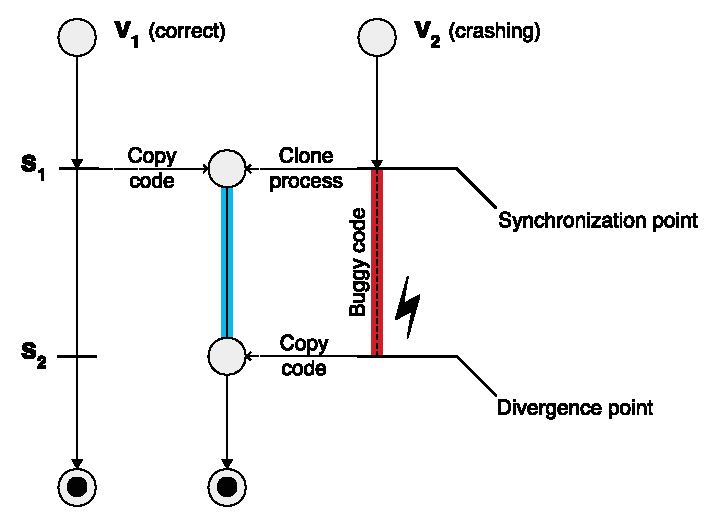
\includegraphics[width=0.5\columnwidth]{safe-updates/figures/strategy}
\caption{\rem's recovery mechanism uses the code of the non-crashing
  version to run through the buggy code.}
\label{fig:solution3}
\end{figure}

%% \begin{enumerate}[label=\emph{S\arabic*}, itemsep=3pt, parsep=3pt]
%% \renewcommand*\labelitemi{\emph{S\arabic*}}
%% \begin{figure}[t]
%%   \centering
%%   \subfloat[Patch state after the crash and continue execution]{
%%     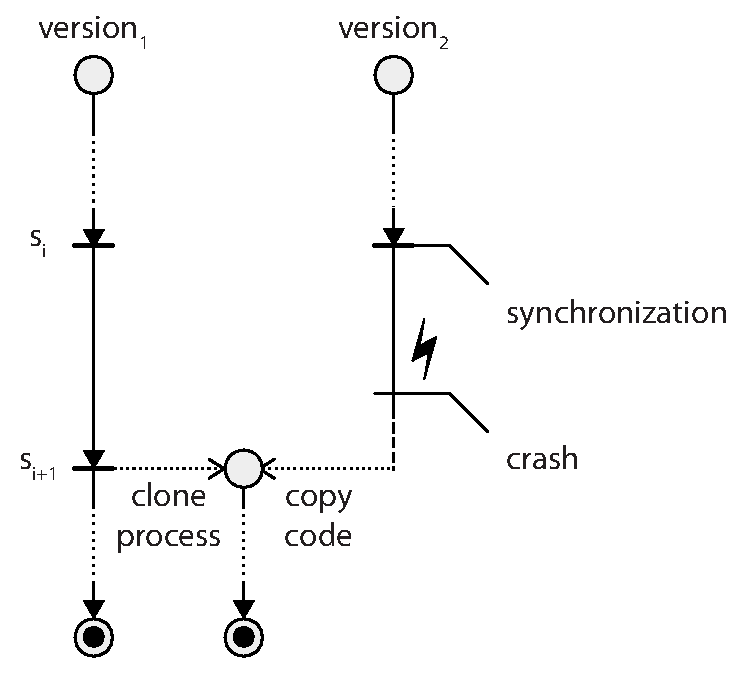
\includegraphics[width=0.45\columnwidth]{safe-updates/figures/solution1}
%%     \label{fig:solution1}
%%   }
%%   \quad
%%   \subfloat[Patch state before the crash and continue execution]{
%%     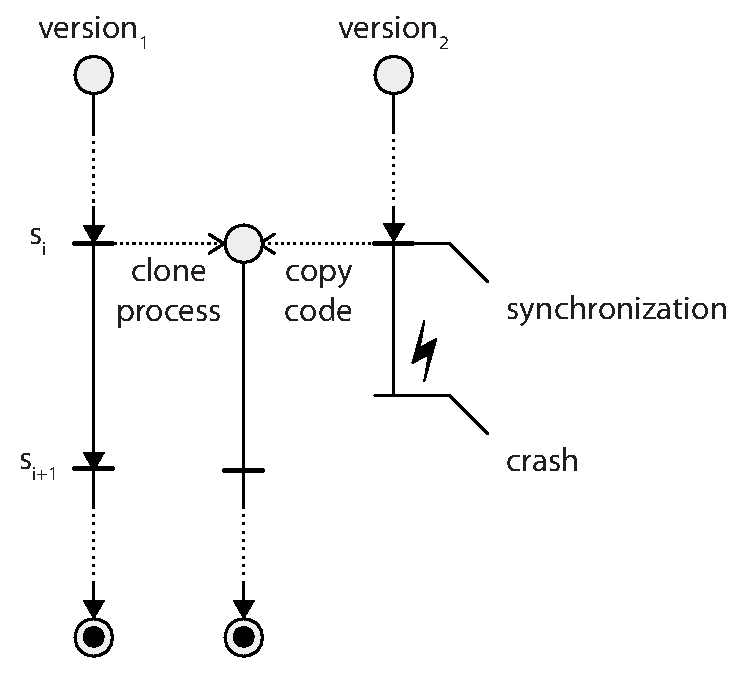
\includegraphics[width=0.45\columnwidth]{safe-updates/figures/solution2}
%%     \label{fig:solution2}
%%   }
%%   \\
%%   \subfloat[Use the code of older version only to run through critical section]{
%%     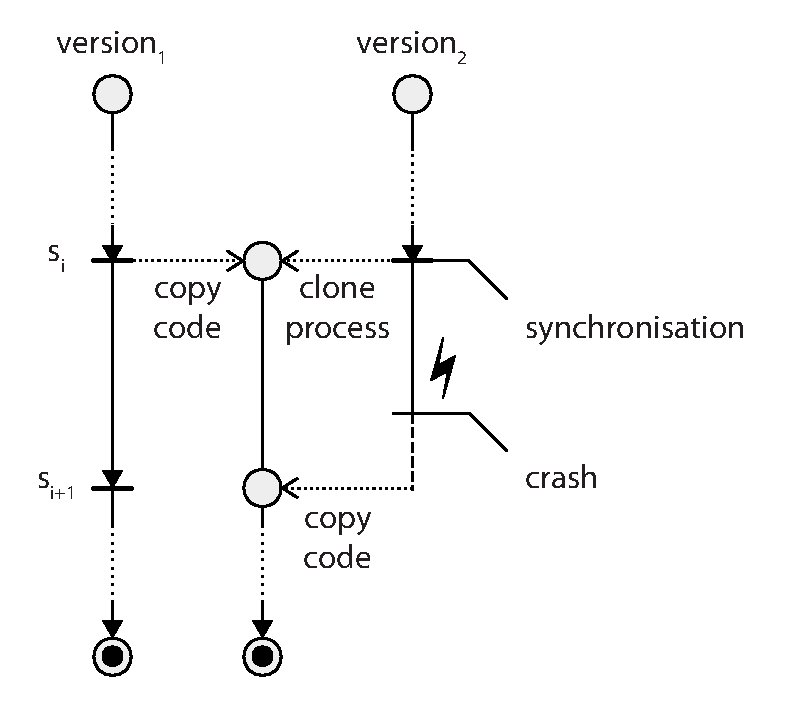
\includegraphics[width=0.45\columnwidth]{safe-updates/figures/solution3}
%%     \label{fig:solution3}
%%   }
%%   \caption{Three solutions for synchronising two divergent versions of
%%   the same application}
%%   \label{fig:solution}
%% \end{figure}

%% \item\label{s1} Clone the correctly executing version to duplicate its state
%%   (\eg memory content, memory mappings) after the crash and replace its
%%   code with the code of the failed version. Then restart both versions and
%%   continue their execution (Figure~\ref{fig:solution1}).

%% \item\label{s2} Clone the correctly executing version to duplicate its state
%%   (\eg memory content, memory mappings) at the last synchronisation point (\ie
%%   creating checkpoint). After the crash, replace the code of this cloned
%%   version with the code of the failed version. Then restart this cloned
%%   version, execute over the \emph{critical section}, and continue execution of
%%   both versions (Figure~\ref{fig:solution2}).

%% \item\label{s3} Clone the failing version to duplicate its state (\eg memory
%%   content, memory mappings) at the last synchronisation point (\ie creating
%%   checkpoint). After the crash, replace the code of this cloned version with
%%   the code of the correctly executing version. Then restart this cloned
%%   version; after the application successfully executes over the \emph{critical
%%   section}, replace the code of the cloned version again with the original
%%   code, and continue its execution (Figure~\ref{fig:solution3}).

%% \end{enumerate}

Our exact recovery mechanism is illustrated in
Figure~\ref{fig:solution3}.  At each system call, \mx creates a
lightweight checkpoint of each version.  This is implemented using the
\lstinline`clone` system call in Linux, which internally uses a
copy-on-write strategy.  
%% As an important optimisation, we omit system
%% calls that can be replayed safely from the last checkpoint, such
%% as \textstt{read}.

As shown in Figure~\ref{fig:solution3}, suppose that the crash happens in
version $v_2$, between system calls $s_1$ and $s_2$.  Then, \rem first restores
$v_2$ at point $s_1$ (\circl{A}), copies $v_1$'s code into $v_2$'s code segment
(\circl{B}), executes over the buggy code using $v_1$'s code (\circl{C}, note
that we are still using $v_2$'s memory state), and then restore $v_2$'s code at
point $s_2$ (\circl{D}).

There are several challenges in implementing this functionality.
First, \rem needs the ability to read and write the application's code
segment.  In the current implementation, we bypass this by linking
together the two application versions after renaming all the symbols
in one of the versions using a modified version of
the \texttt{objcopy}
tool.\footnote{\url{http://sourceware.org/binutils/docs/binutils/objcopy.html}}
However, in the future we plan to implement this transparently by
using the cross-memory attach mechanism used by \mxm.
%% \textstt{pread} and \textstt{pwrite} interface to directly
%% read and write the process memory via the
%% %\textstt{/proc/<pid>/mem} file in the
%% \emph{proc} file system.

%% This functionality has been recently introduced to the Linux kernel in
%% version 2.6.39~\cite{kernel-procmem}; previously, this interface was
%% read-only. This approach imposes only minimal overhead as it allows
%% direct access to the process memory space.

%% The runtime process manipulation functionality is implemented inside
%% \rem, a separate component used by the \mxm monitor. The
%% manipulation itself is driven by the data obtained statically by the
%% \sea analyser before the application has been executed.

Second, \rem needs to modify the contents of the stack in $v_2$.  This is
necessary because the return addresses on the stack frames of $v_2$ still point
to $v_2$'s original code, which was now replaced by $v_1$'s code.  Without also
modifying $v_2$'s stack, any function
\lstinline[language={[x64]Assembler}]`RET` instruction executed between $s_1$
and $s_2$ would most likely veer execution to an incorrect location, since
function addresses are likely to be different across different versions.  Thus,
after \rem replaces $v_2$'s code, it also updates the return addresses on
$v_2$'s stack with the corresponding return addresses in $v_1$, which are
obtained via static analysis (\S\ref{sec:sea}).  Because system calls are
invoked via wrapper functions in C library, this ensures that when $v_2$
resumes execution, it will immediately return to the code in $v_1$.
%% \rem obtains these addresses by analysing $v_1$'s stack at
%% position $s_1$ accessible via checkpoint taken at that point.
%
To implement this functionality, \rem makes use of
the \texttt{libunwind}
library,\footnote{\url{http://www.nongnu.org/libunwind/}} which provides a
portable interface for accessing the program stack, for both x86 and
x86-64 architectures. To actually modify the execution stack of
$v_2$, \rem uses again the \ptrace interface.


Unfortunately, updating the stack return addresses is not sufficient
to ensure that $v_2$ uses $v_1$'s code between $s_1$ and $s_2$, as
$v_2$ may also use function pointers to make function calls.
%% Note that we are still using the $v_2$ memory state. Thereby, $v_2$
%% may still issue a function call to the original code through one of
%% the function pointers.
To handle such cases, \rem inserts breakpoints to the first
instruction of every function in $v_2$'s original code.  Then, when a
breakpoint is encountered, \rem is notified via a \lstinline`SIGTRAP`
signal, and redirects execution to the equivalent function in $v_1$'s
code (which is obtained from the \sea component) by simply changing
the instruction pointer.
%The address of the equivalent function is obtained

Finally, after executing through the buggy code, \rem performs the
same operations in reverse: it redirects execution to $v_2$'s original
code, changes the return addresses on the stack to point to $v_2$'s
functions, and disables all breakpoints inserted in $v_2$'s code.  
The one additional operation that is done at this point is to copy all
the global data modified by $v_1$'s code into the corresponding
locations referenced by $v_2$'s code.  

%\paragraph{Runtime stack analysis and manipulation.}

%% For example, on the x86 architecture, the stack can be easily
%% traversed starting from the top as each stack frame contains frame
%% pointer pointing to the previous stack frame, thereby forming a linked
%% list-like structure. This is not possible on the x86-64 architecture
%% as the frame pointer is no longer stored inside the stack frame.  To
%% traverse the execution stack on this architecture, it is necessary to
%% compute sizes of all functions' stack frames using the stack usage
%% information stored in the \texttt{UNWIND\_CODE} section, which is a
%% part of the ELF binary file. This logic is implemented by the
%% \texttt{libunwind} library, which provides API to unwind the stack
%% independent of the target platform.

%The necessary information about the stack location (\ie address range) and
%page mapping are obtained through the \emph{proc} file system; in particular
%the \textstt{/proc/<pid>/maps} and \textstt{/proc/<pid>/pagemap} files.

Note that \mx cannot currently handle major modifications to the
layout of the data structures used by the code, including individual
stack frames.  While this still allows us to support several common
software update scenarios, in future work we plan to improve the
system with the ability to perform full stack
reconstruction~\cite{upstare} and automatically infer basic data
structure changes at the binary-level~\cite{data-struct-digging}.
%% to identify changes to function names and sequences of function calls
%% (e.g., via clone detection techniques~\cite{cp-miner06,deckard07}),


Our approach of using the code of the non-crashing version to survive failures
in the crashing version may potentially leave the recovered version in an
inconsistent state. However, \mx is able to discover most internal state
inconsistencies by checking whether the two versions have the same external
behaviour after recovery. When the behaviour of the recovered version starts to
differ, \mx will immediately discard it and continue with only one version. The
discarded version can be later restarted at a convenient synchronisation point.
This restarting functionality is not currently implemented in \mx, but we plan
to add it as a future extension.

%Our approach of using the code of the non-crashing version to survive
%failures in the crashing one may leave the application in an
%inconsistent state, and thus may not be applicable for application in
%which absolute correctness and a fail-fast approach are more important
%than allowing the application to survive errors.  However, \mx is
%usually able to discover most internal state inconsistencies, since it
%regularly checks if the two versions have the same external
%behaviour. (See \S\ref{sec:discussion} for an extended discussion.)

\subsection{Binary static analysis}
\label{sec:sea}

%% \begin{table*}[t]
%% \centering 
%% \begin{tabular}{ccc}
%%   \hline
%%   Library calls in $\mathrm{version}_1$ & Library calls in $\mathrm{version}_2$ &
%%   System calls within the library \\
%%   \hline
%%   \texttt{<0xdeadbe5a>} & \texttt{<0xdeadbe8e>} &
%%   [\texttt{<0x77ff2c>}, \texttt{<0x77ffae>}] \\
%%   \texttt{<0xdeadabf5>} & \texttt{<0xdeadac34>} &
%%   [\texttt{<0x782bae>}] \\
%%   \vdots & \vdots & \vdots \\
%% \end{tabular}
%% \caption{Addresses of library function calls, and system calls invoked from
%% within these functions.}
%% \label{tab:syscall_table}
%% \end{table*}

The \sea component statically analyses the binaries of the two
versions to obtain information needed at runtime by the \rem
component.  \sea is invoked only once, when the multi-version
application is assembled from its component versions.
%% As mentioned in \sref{sec:rem}, we currently link together the
%% two application versions after renaming all the symbols in one of them
%% using a modified copy of the \textstt{objcopy} tool, although in the
%% future we plan to do this linking dynamically by directly changing the
%% code segment in each version.

The main goal of \sea is to create several mappings from the code of
one version to the code of the other.  First, \sea extracts the
addresses of all function symbols
in one version and maps them to the
addresses of the corresponding functions in the other version.  This
mapping is used by \rem to handle calls performed via function
pointers (\S\ref{sec:rem}).

Second, \sea computes a mapping from all possible return addresses in
one version to the corresponding return addresses in the other version.  In
order to allow for code changes, this mapping is done by computing an
ordered list of all possible return addresses in each function.  For
example, if function \lstinline`foo` in $v_1$ performs call instructions
at addresses \lstinline`0xabcd0000` and \lstinline`0xabcd0100`, and
function \lstinline`foo` in $v_2$ performs call instructions at
addresses \lstinline`0xdcba0000` and \lstinline`0xdcba0400`, then \sea
will compute the mapping \texttt{\{0xabcd0005 $\rightarrow$
0xdcba0005, 0xabcd0105 $\rightarrow$ 0xdcba0405\}} (assuming each call
instruction takes 5 bytes).  This mapping is then used by \rem to
rewrite return addresses on the stack.

%% These data are gathered by the \sea analyser component which
%% implements static analysis of binary executables to extract all
%% necessary addresses and provide them to other components inside our
%% system. The format used for storing these data is represented by a
%% \emph{call table}. For each version, this table contains addresses of
%% all calls to shared library functions together with the list of all
%% system calls addresses invoked within these library functions, as can
%% be seen in Table~\ref{tab:syscall_table}.

%% For example, the first line of this table represents a call to a
%% library function which does two system calls, while second line
%% represents a function call which does only one system call.

To construct these tables, \sea first needs to extract the addresses
of all function symbols and then disassemble the code for each
individual function in order to locate the call instructions within
them.  The implementation is based on the \texttt{libbfd}
and \texttt{libopcodes} libraries, which are 
part of the
\gnu \binutils suite.\footnote{\url{http://www.gnu.org/software/binutils/}}
To obtain the addresses of all function symbols defined by the
program, \sea uses \texttt{libbfd} to extract the static and dynamic
symbol tables and relocation tables.  To disassemble individual
functions, \sea uses the \texttt{libbf}
library~\cite{kwan:libbf}, built on top of \texttt{libopcodes}.

%% Disassembled machine code is stored in a graph-like structure where
%% individual instructions represents vertices and edges between these
%% vertices represents the control flow. 

%% \paragraph{System call identification.}
%% \sea implementation uses the disassembler to obtain machine
%% code of each individual function and iterates over its instructions
%% (traversing the instruction graph) to identify basic blocks and locate
%% system call instructions within the code these functions.

%% To locate system calls within shared library function calls,
%% \sea first needs to obtain the set of exported library
%% functions and system calls within these functions using the above
%% described approach. Then, \sea analyses the application binary
%% itself and locates all function calls to the shared library using the
%% information extracted from relocation and procedure lookup tables
%% contained in ELF binaries.

%% Results of this analysis are stored in a hash table and tree structure
%% to allow quick access eliminating any unnecessary overhead when these
%% information are accessed during runtime. These data are then used to
%% construct the already described \emph{call table}, before the
%% application itself is executed.

%% \subsection{Limitations and Future Work}
%% \label{sec:limitations}
%% \input{limitations}

\section{Reliability Evaluation}
\label{sec:reliability-evaluation}

To evaluate our approach, we show that \mx can survive crash bugs in several
real applications (\S\ref{sec:surviving}). We then examine the question of how
far apart can be the versions run by \mx (\S\ref{sec:bounds}), and discuss
\mx's performance overhead (\S\ref{sec:performance}).

\subsection{Fault recovery}
\label{sec:surviving}

We have evaluated \mx using a set of bugs in three applications: \gnu
\coreutils, \redis and \lighttpd. We discuss each application in turn below.

\subsubsection{\gnu \coreutils}
\label{sec:coreutils}

\begin{table}[t]
\begin{center}
\caption{Utilities from \gnu \coreutils, the crash bugs used, and the 
versions in which these bugs were introduced and fixed.  We group
together utilities affected by the same or similar bugs.}
\begin{tabular}{lll}
\toprule
\textsc{Utility} & \textsc{Bug description} & \textsc{Bug span} \\
\midrule
\mdsum & \multirow{2}{*}{Buffer underflow} & \multirow{2}{*}{v5.1 -- v6.11} \\
\shasum & & \\
\midrule
\mkdir & \multirow{2}{*}{\textstt{NULL}-pointer dereference} & \multirow{2}{*}{v5.1 -- v6.11} \\
\mkfifo & & \\
\mknod & & \\
\midrule
\cut & Buffer overflow & v5.3 -- v8.11 \\
\bottomrule
\end{tabular}
\label{tbl:cu-bugs}
\end{center}
\end{table}

As an initial evaluation of \mx's ability to survive crashes, we have used
applications from the \gnu \coreutils utility
suite,\footnote{\url{http://www.gnu.org/software/coreutils/}} which provides
the core user-level environment on most UNIX systems.  We have selected a
number of bugs reported on the \coreutils mailing list, all of which trigger
segmentation faults.  The bugs are described in Table~\ref{tbl:cu-bugs},
together with the utilities affected by each bug and the versions in which they
were introduced and fixed.

The bug affecting both \mdsum and \shasum utilities introduced in 5.1 and later
fixed in 6.11 caused a crash due to buffer underflow when checking an invalid
BSD-style input. Another bug we have considered affected \mkdir, \mkfifo and
\mknod utilities; this bug, which was reported in 6.10 and fixed in 6.11
resulted in crash when diagnosing invalid context.  Finally, the bug affecting
\cut utility, introduced in 5.3 and later fixed in 8.11, resulted in segfault
when using large unbounded range. 

For all these bugs, we configured \mx to run the version that fixed the bug
together with the one just before.  (we could have also run the version that
introduced the bug with the one just before, but we could not immediately tell
where the bug was introduced, and we cannot build versions earlier than 6.10
due to changes in GCC and GNU C library).  \mx successfully intercepted the
crash and recovered the execution by using the strategy described in
\sref{sec:rem}.

We discuss below the bug in the \cut utility (used to remove sections from each
line of file), triggered by the following invocation:

\begin{lstlisting}[numbers=none,breaklines=true,xleftmargin=0pt,language=bash]
cut -c1234567890- --output-d=: foo
\end{lstlisting}

This bug is triggered by the conditional statement on line~\ref{line:cond}:

\begin{lstlisting}[firstnumber=525]
if (output_delimiter_specified /*@\label{line:cond}@*/
    && !complement
    && eol_range_start && !is_printable_field (rsi_candidate))
\end{lstlisting}

This code uses the lower bound of the size of the printable field
vector; however, when calculating the size of this vector, ranges going
to the end of line (\ie \lstinline`0-`) are not considered eventually
resulting in invalid memory access. 
% The bug is caused by a buffer overflow whose root cause is the
% incorrect calculation of the size of a dynamically allocated buffer
% used internally by \cut.
When \mx intercepts this bug, it uses the
last checkpoint to recover the execution of the crashing version. This
checkpoint is taken after the \textstt{brk} system call triggered by
the \textstt{malloc} call that allocates the buffer. 
% in function \textstt{bindtextdomain} on line~\ref{line:bind}.
% \begin{lstlisting}[firstnumber=767]
% bindtextdomain (PACKAGE, LOCALEDIR); /*@\label{line:bind}@*/
% \end{lstlisting}
The recovered process uses the code of the other version to correctly
calculate the size of the field vector and switches back to the original
code during the allocation of this buffer as
%code during the allocation of this buffer on line~\ref{line:alloc} as
function \textstt{xzalloc} triggers \textstt{mmap64} system call, just
before executing the conditional statement on line~\ref{line:cond},
which originally triggered the bug.

\subsubsection{\redis}
\label{sec:redis}

Below, we describe how \mx can survive the \redis bug described in
Section~\ref{multi-version:scenarios} while running in parallel the \redis
revision \textstt{a71f072f} (\textit{the old version}, just before the bug was
introduced) with revision \textstt{7fb16bac} (\textit{the new version}, just
after the bug).  \mx first invokes \sea to perform a static analysis of the two
binaries and construct the mappings described in \sref{sec:sea}.  Then, \mx
invokes the \mxm monitor, which executes both versions as child processes and
intercepts their system calls.

When the new version crashes after issuing the problematic
\textstt{HMGET} command, \mxm intercepts the \textstt{SIGSEGV} signal
which is sent to the application by the operating system.  At
this point, \rem starts the recovery procedure.  First, \rem sends a
\textstt{SIGKILL} signal to the new version to terminate it.  It then
takes the last checkpoint of the new version, which was taken at the
point of the last invoked system call, which in this case is an
\textstt{epoll\_ctl} system call.  Then, \rem uses the information
provided by \sea to rewrite the stack of the new version, as detailed
in \sref{sec:rem}.  In particular, \rem replaces the return
addresses of all functions in the new version with the corresponding
addresses from the old version. The stack rewriting itself however is not
enough. The newer version can still use function pointers, which are part of
the replica state, to invoke the original code. To prevent this situation, \rem
inserts breakpoints at the beginning of all the functions in the code of the
new version (to intercept indirect calls via function pointers), and then
finally restores the original processor registers of the checkpointed process
and restarts the execution of the (modified) new version.

Since the checkpoint was performed right after the execution of the system
call \textstt{epoll\_ctl}, the first thing that the code does is to
return from the \textstt{libc} wrapper that performed this system
call.  This in turn will return to the corresponding code in the old
version that invoked the wrapper, since all return addresses on the
stack have been rewritten.  From then on, the code of the old version
is executed (but in the state of the new version), until the first
system call is intercepted.  In our example, the old and the new
versions perform the same system call (and with the same arguments),
so \rem concludes that the two processes have re-converged, and thus
restores back the code of the new version by performing the steps
above in reverse, plus the additional step of synchronising their
global state (see \S\ref{sec:rem}).  Finally, the control is handed
back to the \mxm monitor, which continues to monitor the execution of
the two versions.

\subsubsection{\lighttpd}
\label{sec:lighttpd}

To evaluate \mx on \lighttpd, we have used two different crash bugs.
The first bug is the one described in detail in
Section \ref{multi-version:scenarios}, related to the ETag and compression
functionalities.  As previously discussed, the crash is triggered by a
very small change, which decrements the upper bound of a \textstt{for}
loop by one.  \mx successfully protects the application against this
crash, and allows the new version to survive it by using the code of
the old version.

The other crash bug we reproduced affects the URL rewrite
functionality.\footnote{\url{http://redmine.lighttpd.net/projects/lighttpd/issues/2140}}
This is also caused by an incorrect bound in a \lstinline`for` loop.
More precisely, the loop: 

\begin{lstlisting}[numbers=none,breaklines=true,xleftmargin=0pt]
for (k=0; k < pattern_len; k++)
\end{lstlisting}

\noindent should have been:

\begin{lstlisting}[numbers=none,breaklines=true,xleftmargin=0pt]
for (k=0; k@+1@ < pattern_len; k++)
\end{lstlisting}

The bug seems to have been present since the very first version
added to the repository.  It was reported in December 2009, and
fixed one month later.  As a result, we are running \mx using the last
version containing the bug together with the one that fixed it.  While
this bug does not fit within the pattern targeted by \mx (where a
newer revision introduces the bug), from a technical perspective it is
equally challenging.  \mx is able to successfully run the two versions
in parallel, and help the old version survive the crash bug.

%The bug \#1601 affects the HTTP redirection functionality, in particular
%the \texttt{\%n} substitution with condition substring. This functionality has
%been introduced in revision \texttt{510}. However, there is an incorrect
%comparison in one of the conditions which causes segmentation fault when
%appending matched parts to buffer if there was no matching regular expression.
%The affected code can be seen in Listing~\ref{lst:510}.

%\begin{lstlisting}[label=lst:510, caption={Original correct version of the function}]
%cond_cache_t *cache = &con->cond_cache[dc->context_ndx];
%if (n > cache->patterncount) {
  %return 0;
%}
%\end{lstlisting}

%The fix to this bug consists of a single changed line as can be seen in
%Listing~\ref{lst:2138} and has been incorporated in revision \texttt{2138}, yet
%this bug remained undetected for nearly three years (August 8, 2005 --- March
%26, 2008) rendering \lighttpd webserver vulnerable to attack.

%\begin{lstlisting}[label=lst:2138, caption={Refactored failing version of the function}]
%cond_cache_t *cache = &con->cond_cache[dc->context_ndx];
%if (n >= cache->patterncount) {
  %return 0;
%}
%\end{lstlisting}

Both \lighttpd bugs \#1601 and \#2140 are very simple---their fix
consist of a single character---yet still they made \lighttpd server
vulnerable to a potential attack. \mx can not only handle the crash,
but also successfully recover the failing version in both cases.

\subsection{Ability to run distant versions}
\label{sec:bounds}

\begin{table}
\begin{center}
\caption{The maximum distance in number of revisions, and the time span
  between the revisions that can be run by \mx for each bug.}
\begin{tabular}{lcc}
\toprule
\textsc{Application Bug} & \textsc{Max distance} & \textsc{Time span} \\
\midrule
\lighttpd \#2169   & \maxDistLighttpdOne & \timeSpanLighttpdOne \\
\lighttpd \#2140   & \maxDistLighttpdTwo & \timeSpanLighttpdTwo \\
\redis \#344       & \maxDistRedis & \timeSpanRedis \\
%md5sum          & \maxDistMdsum & \timeSpanMdsum \\ \hline
\bottomrule
\end{tabular}
\label{tbl:bug-bounds}
\end{center}
\end{table}

In the previous sections, we have shown how \mx can help software
survive crash bugs, by running two \textit{consecutive} versions of an
application, one which suffers from the bug, and one which does not.
%
One important question is how far apart can be the versions run
by \mx.  To answer this question, we determined for each of the bugs
discussed above the most distant revisions that can be run together to
survive the bug.  

For the \coreutils benchmarks, we are able to run versions which are
hundreds of revisions apart: \maxDistMdsum~revisions (corresponding to
\timeSpanMdsum of development time) for the \mdsum/\shasum bug; 
\maxDistMkdir~revisions (\timeSpanMkdir of development time) for the 
\mkdir/\mkfifo/\mknod bug; and \maxDistCut~revisions (\timeSpanCut 
of development time) for the \cut bug.

The most distant versions for the first \lighttpd bug are
approximately two months apart and have \maxDistLighttpdOne~revisions
in-between, while the most distant versions for the second
\lighttpd bug are also approximately two months apart but have only
\maxDistLighttpdTwo~revisions in-between.  Finally, the most distant
versions for the \redis bug are \maxDistRedis~revisions
and \timeSpanRedis apart.  

Of course, it is difficult to draw any general conclusions from only
this small number of data points.  Instead, we focus on understanding
the reasons why \mx could not run farther apart versions for the bugs
in \lighttpd and \redis (we ignore \coreutils, for which we can run
very distant versions).
%% For the \coreutils bugs, the lower bound is the earliest
%% version that we could build and run on our machine (v6.10).  The
%% upper-bound for 
%
For \lighttpd issue \#2169, the lower bound is defined by a revision
in which a pair of \textstt{geteuid()} and \textstt{getegid()} calls
are replaced with a single call to \textstt{issetugid()} to
allow \lighttpd to start for a non-root user with GID~0.  \mx 
%cannot run this revision together with the one before it, because it 
currently does not support changes to the order of system calls, but we believe
this limitation could be overcome by using peephole-style
optimisations~\cite{dragon-book}, which would allow \mx to recognise
that the pair \textstt{geteuid()} and \textstt{getegid()} could be
matched with the call to \textstt{issetugid()}.  The upper bound
for \lighttpd issue \#2169 adds a \textstt{read} call to
\textstt{/dev/[u]random}, in order to provide a better entropy
source for generating HTTP cookies.  This additional \textstt{read}
call changed the sequence of system calls, which \mx cannot
handle. \looseness=-1

For \lighttpd issue \#2140, both the lower and the upper bounds are
caused by a change in a sequence of \textstt{read()} system calls.  We
believe this could be optimised by allowing \mx to recognise when two
sequences of read system calls are used to perform the same overall
read.

%% Lower bound: the fix consists of request parser changes which resulted
%% in different sequence of \textstt{read()} system calls. The different
%% sequence of \textstt{read()} calls also marked the upper bound in this
%% case, defined by revision \lighttpdTwoUB. In this revision, the way in
%% which input connection buffer is being filled has changed, fixing
%% issue \#2147 and CVE-2010-0295 vulnerability.

For the \redis bug, the lower bound is given by the revision in which the
\textstt{HMGET} command was first implemented.  Since there was no support for
\textstt{HMGET} before that version, \mx has no way to survive the crash caused
by invoking \textstt{HMGET} with a wrong type (see \S\ref{sec:redis}).  The
upper bound is defined by a revision which changes the way error responses are
being constructed and reported, which results in a very different sequence of
system calls.

%% , including the call on line
%% \ref{line:report-error2} in Listing~\ref{lst:refactored}, resulting in
%% different sequence of system calls.

%% \todo{explain that all of these changes are minor and some of them could be
%% very well handled by using window-based/peep-hole approach}

\subsection{Performance Overhead}
\label{sec:performance}

\begin{figure}[!t]
\centering
\includegraphics[width=\textwidth]{safe-updates/graphs/spec2006}
\caption{Normalised execution times for the \spec benchmark suite running under
\mx.}
\label{fig:spec}
\end{figure}

We ran our experiments on a four-core server with 3.50~GHz Intel
Xeon E3-1280 and 16~GB of RAM running 64-bit Linux v3.1.9.

\paragraph{\spec.}
To measure the performance overhead of our prototype, we first used
the standard \spec\footnote{\url{http://www.spec.org/cpu2006/}}
benchmark suite.  Figure~\ref{fig:spec} shows the performance of \mx
running two instances of the same application in parallel, compared to
a native system. The execution time overhead of \mx varies
from \minOverSPEC to \maxOverSPEC compared to executing just a single
version, with the geometric mean across all \numSPECbench benchmarks at
\avgOverSPEC. This result is comparable with previous work using multi-variant
execution that used SPEC CPU to measure performance~\cite{orchestra09} (even
though this work used SPEC~CPU2000 which has already been retired).

%% The overhead varies from \minRedisOver to \maxRedisOver depending
%% on the operation being performed. This is the worst case overhead
%% we have seen among all tested application and comes mainly from the
%% fact that \redis is an in-memory database optimised for maximum
%% bare-hardware performance and is very sensitive to any additional
%% software layers.  Even a state-of-the-art hypervisor can incur an
%% $n$-fold slowdown, so the relatively high measure overhead is
%% therefore unsurprising.

\paragraph{\gnu~\coreutils.} The six \coreutils applications discussed in 
\sref{sec:coreutils} are mostly used in an interactive fashion via the
command-line interface (CLI). For such applications, a high performance
overhead is acceptable as long as it is not perceptible to the user;
prior studies have shown that response times of less than 100ms
typically feel instantaneous~\cite{card:human_proc}. In many common use
cases (\eg creating a directory, or using \cut on a small text file),
the overhead of \mx was imperceptible---\eg creating a directory takes
around \avgMkdirNative natively and \avgMkdirMx with \mx. For the three
utilities that process files, we calculated the maximum file size for
which the response time with \mx stays under the 100ms threshold.  For
\cut, the maximum file size is \cutCutoffSize (with an overhead of
\cutCutoffOver), for \mdsum \mdsumCutoffSize (\mdsumCutoffOver
overhead), and for \shasum \shasumCutoffSize (\shasumCutoffOver
overhead).



\paragraph{\redis and \lighttpd.} To measure the performance overhead for \redis, 
we used
the \redisbenchmark\footnote{\url{http://redis.io/topics/benchmarks}}
utility, which is part of the standard \redis distribution and
simulates \textstt{GET}/\textstt{SET} operations done by $N$ clients
concurrently, with default workload.  For \lighttpd, we used the
\httpload\footnote{\url{http://www.acme.com/software/http_load/}}
multiprocessing test client that is also used by the \lighttpd
developers.  Both of these standard benchmarks measure the end-to-end
time as perceived by users.  As a result, we performed two sets of
experiments: (1) with the client and server located on the same
machine, which represents the worst case performance-wise for \mx; and
(2) with the client and server located on different continents (one in
England and the other in California), which represents the best case.

The overhead for \redis varies, depending on the operation being
performed, from \minRedisRemote to \maxRedisRemote in the remote
scenario, and from \minRedisOver to \maxRedisOver in the local
scenario.  The overhead for \lighttpd varies from \minLighttpdRemote
to \maxLighttpdRemote in the remote scenario, and
from \minLighttpdOver to \maxLighttpdOver in the local scenario.
Despite the relatively large overhead in the local experiments, the
remote overhead is negligible because times are dominated by the
network latency (which in our case is over $150$ms).

As a result, we believe \mx is most suitable for scenarios for which
its execution overhead does not degrade the performance of the
end-to-end task, such as the remote \redis and \lighttpd scenarios
discussed above, or interactive tasks such as those performed using
command-line utilities, where users would not notice the overhead as
long as the response time stays within a certain range.

%% \mx's performance overhead is strongly correlated with the frequency of
%% system calls that have to be intercepted.  Therefore, we could also
%% imagine \mx being automatically turned on and off during execution,
%% depending on the frequency of system calls experienced by the
%% application.

Finally, we would like to emphasise that our current prototype has not
been optimised for performance, and we believe its overhead can still
be significantly reduced.  
%% There are multiple strategies we plan to explore in future
%% work. First,
For example, we could synchronise versions at a coarser granularity,
by using an epoch-based approach~\cite{compl-schedules11}, or we could
improve our checkpointing mechanism by implementing it as a loadable
kernel module that only stores the part of the state needed for
recovery~\cite{flashback}.

%% and only checkpoint at epoch boundaries.  To make this approach viable, we also
%% need to record system calls in each epoch, so that they can be
%% replayed during recovery. Second, 

%% instead of using \textstt{clone}
%% directly, we could implement the checkpointing functionality as a
%% loadable kernel module and only store the part of the state needed for
%% recovery as in~\cite{flashback}. Finally, we could explore the
%% possibility of not intercepting system calls in certain parts of the
%% code that were previously shown to be safe and do not need to be
%% replicated across multiple versions (\eg similarly
%% to~\cite{onlinevalidation}).

%The measured overhead is higher than
%for the SPEC~CPU2006 benchmarks (with a slowdown of up to \maxRedisOver
%for some operations in \redis) and we are currently investigating the
%reasons for this slowdown.

%First, we could to synchronise versions at a coarser
%granularity, by using a window/epoch approach~\cite{compl-schedules11},
%and by performing certain synchronisations at the level of shared
%library calls.  Second, we could explore the possibility of not
%intercepting system calls in certain parts of the code that were
%previously shown to be safe and do not need to be replicated across
%multiple versions.  Finally, we could decrease the checkpointing
%overhead, by performing them at a lower frequency, and record the
%external behaviour since the last checkpoint, so that it can be
%successfully replayed during recovery (\eg as in Rx~\cite{rx}).

\begin{figure}[ht]
\begin{center}
\includegraphics[angle=270,width=\textwidth]{safe-updates/graphs/syscall}
\caption{Number of system calls made on average each second during the
execution of SPEC~CPU2006 benchmark suite, measured using \textstt{strace}
tool.}
\label{fig:syscall}
\end{center}
\end{figure}

We also examined how frequency of system calls affects the performance
overhead of application executed on top \mx. Figure~\ref{fig:syscall} shows
the average number of system calls during the execution of SPEC~CPU2006.
Rather surprising result is the fact that \textsf{452.libquantum}, even though having
the largest run time overhead had the lowest average number of system calls.
On the hand, the performance overhead of \textsf{400.perlbench}, despite having the
highest average number system, was bellow average. \todo{What is the conclusion here?}

% For example, as we discuss in related work, our
% monitor \mxm is very similar to the monitor used by
% Orchestra~\cite{orchestra09}, which by employing various optimisations
% manages to obtain an average overhead of only about 15\% when
% synchronising two program variants at the level of system calls.  In
% terms of checkpointing, the Rx system~\cite{rx} implements a similar
% approach based on the Linux copy-on-write mechanism, and which through
% various optimisations manages to achieve a performance penalty of less
% than 5\% when checkpointing every 200 milliseconds.

\section{Discussion}
\label{safe-updates:discussion}

This section discusses in more detail the scope of our approach with
regard to the type of software updates suitable to multi-version
execution and the different trade-offs involved.

%% This section discusses in more detail the scope of our approach
%% with regard to (1) the type of applications and code changes that
%% could benefit most from our approach, and (2) the trade-off between
%% availability/reliability/availability and strict
%% correctness/performance/energy consumption.

\paragraph{Types of code changes} In order for \mx to be successful, the
external behaviour of the versions that are run in parallel has to be similar
enough to allow us to synchronise their execution.  Our empirical study in
\S\ref{evolution:external} shows that changes to the external behaviour of
an application are often minimal, so our approach should work well with
versions that are not too distant from one another.  Similarly, our system
relies on the assumption that versions re-converge to the same behaviour after
a divergence.  As a result, we believe \mx would be a good fit for applications
that perform a series of mostly independent requests, such as network servers.
These applications are usually structured around a main dispatch loop, which
provides a useful re-convergence point.  Our approach is also suitable to local
code changes, which have small propagation distances, thus ensuring that the
different versions will eventually re-converge to the same behaviour.

\paragraph{Trade-offs involved} Our approach is targeted toward scenarios
where the availability, reliability and security of a software system is more
important than strict correctness, high performance and low energy consumption.  

In terms of correctness guarantees, \mx is similar to previous approaches such
as failure oblivious computing~\cite{fo} which may sacrifice strict correctness
for increased availability and security (see \S\ref{sec:rem} for details
regarding possible problems caused by \mx).  However, \mx alleviates this
problem by using a previously correct piece of code to execute through the
crash, and by discovering most potential problems by regularly checking if the
two versions have the same external behaviour.  Finally, note that \mx always
reverts to running a single version when a non-resolvable divergence is
detected.

%% is never worse than simply using one version of the software: if a
%% non-crashing divergence is detected, \mx can simply continue execution
%% with a single program version.

\paragraph{CPU utilisation} \mx incurs a performance overhead, as discussed in
\sref{sec:performance}.  In our experience, \mx is readily deployable to
interactive applications such as command-line utilities, text editors and other
office tools, where the performance degradation is not noticeable to the user.
We believe it is also applicable to server applications where availability is
more important than high performance.  \mx is not applicable to patches that
fix performance bugs, as the system runs no faster than the slowest
version.

Our approach of using idle CPU time to run additional versions also increases
energy consumption.  However, it is interesting to note that idle CPUs are not
``free'' either: even without considering the initial cost of purchasing the
cores left idle, an energy-efficient server consumes half its full power when
doing virtually no work---and for other servers, this ratio is usually much
worse~\cite{barroso2007}.
% and therefore might not be applicable to energy-constrained devices
%such as smartphones.

\paragraph{Deployment strategy} While our approach eases the decision of
applying a software update---as incorporating a new version would never
decrease the security and reliability of the overall multi-version
application---the number of versions that can be run in parallel is limited,
being dictated by the number of available resources (\eg the number of
available CPU cores).  As a result, we need a deployment strategy to decide
what versions to use.  For example, we could always run the last $N$ released
versions (where $X$ is the number of available resources), or we could always
keep a one-year old version, etc.  This thesis focuses on techniques for
allowing multiple versions to successfully coordinate their parallel execution,
but in future work we plan to explore deployment strategies in more detail.

\section{Summary}
\label{safe-updates:summary}

Software updates are an important part of the software development and
maintenance process. Unfortunately, they also present a high failure risk, and
many users refuse to upgrade their software, relying instead on outdated
versions, which often leave them exposed to known software bugs and security
vulnerabilities.

In this chapter, we have presented \mx, a multi-version execution system for
improving the software update process. Whenever a new program update becomes
available, instead of upgrading the software to the newest version, we run the
new version in parallel with the old one, and carefully synchronise their
execution to create a more secure and reliable multi-version application.

\mx supports off-the-shelf Linux applications and our evaluation has shown that
it can be applied successfully to several real applications such as \coreutils,
\lighttpd, and \redis.

